\documentclass[journal,12pt,twocolumn]{IEEEtran}
\makeatletter
\@addtoreset{figure}{problem}
\makeatother
\usepackage{graphicx}
\usepackage{pifont}
\usepackage{graphicx,float}
\usepackage{listings}
\usepackage{hyperref}
\hypersetup{
    colorlinks=true,
    linkcolor=blue,
    filecolor=magenta,      
    urlcolor=cyan,
}
 
\urlstyle{same}
%\usepackage{epsfig} % for postscript graphics files
%\usepackage{mathptmx} % assumes new font selection scheme installed
%\usepackage{times} % assumes new font selection scheme installed
%\usepackage{amsmath} % assumes amsmath package installed
%\usepackage{amssymb}  % assumes amsmath package installed

\title{\LARGE \bf
Healthcare Application using Ethereum Blockchainhain Installation Guide
}

\author{ \parbox{3 in}{\centering P. V. Vineeth Kumar,
         Student of Electrical Engineering\\
         IIT Hyderabad}
         \hspace*{ 0.5 in}
         \parbox{3 in}{ \centering Dr.GVV Sharma,
         Faculty in Department of Electrical Engineering \\
         IIT Hyderabad}
}

\begin{document}



\maketitle
\thispagestyle{empty}
\pagestyle{empty}


%%%%%%%%%%%%%%%%%%%%%%%%%%%%%%%%%%%%%%%%%%%%%%%%%%%%%%%%%%%%%%%%%%%%%%%%%%%%%%%%
\begin{abstract}

This manual provides a step-by-step procedure for deploying a web application into the private Ethereum blockchain network by installing Ethereum geth client and interacting with the Ethereum blockchain network. It also discuss smart contracts and their deployment.
	
\end{abstract}


%%%%%%%%%%%%%%%%%%%%%%%%%%%%%%%%%%%%%%%%%%%%%%%%%%%%%%%%%%%%%%%%%%%%%%%%%%%%%%%%
\section{INTRODUCTION}

This case study explores the use of blockchain enabled technology to achieve distributed and trustworthy transaction handling between two ethereum nodes with a User Interface  as the medium.

\section{SYSTEM CONFIGURATION}

\subsection{Smart Contract Platform}

The framework discussed here is based on the Ethereum Smart Contract Platform.
At its simplest, Ethereum is an open software platform based on blockchain technology that enables developers to build and deploy decentralized applications.\\
Like Bitcoin, Ethereum is a distributed public blockchain network. Although there are some significant technical differences between the two, the most important distinction to note is that Bitcoin and Ethereum differ substantially in purpose and capability. Bitcoin offers one particular application of blockchain technology, a peer to peer electronic cash system that enables online Bitcoin payments. While the Bitcoin blockchain is used to track ownership of digital currency (bitcoins), the Ethereum blockchain focuses on running the programming code of any decentralized application.

\subsection{What is Smart Contract?}

Smart contract is just a phrase used to describe computer code that can facilitate the exchange of money, content, property, shares, or anything of value. When running on the blockchain a smart contract becomes like a self-operating computer program that automatically executes when specific conditions are met. Because smart contracts run on the blockchain, they run exactly as programmed without any possibility of censorship, downtime, fraud or third party interference.

\section{HARDWARE AND SOFTWARE}

We considered a case with two personal computers. One of the PC is a Vendor Node and another one is the passive node. We can use both of them as miners or we can restrict one node as non-miner. \\

On each device, a geth client(a command line interface implemented in the Go language was installed to transform them into an Ethereum node. With the geth clients, we created an ethereum account for each node and configured these networks to form a private blockchain network.In this network, Vendor Node plays the role of miner and the Passive Node is the lightweight ethereum node that play the function of sending transactions.

\subsection{INSTALLING ETHEREUM CLIENT} 
The setup of the Vendor Node and Passive Node requires the following hardware:
\begin{itemize}
  \item A Personal Computer with atleast 1 TB hard 			disk
  %\item SD card of atleast 16Gb
  \item A LAN cable
  \end{itemize}
Open the terminal and type the following commands to install an Ethereum client(geth-Go Ethereum)
\begin{itemize}
\item \$ sudo apt-get install software-properties-common
\item  \$ sudo add-apt-repository -y  ppa:ethereum/ethereum
\item \$ sudo apt-get update
\item \$ sudo apt-get install ethereum\\

Check the version of Geth:\\
\textbf{pi\$ geth version}\\
\end{itemize}


\subsection{SET UP A PRIVATE CHAIN:MINER NODES}
Our private chain needs miners in order to validate and propagate blocks of transactions within the blockchain. Miners will also be used to generate ether to pay for the gas required to process transactions on the Ethereum blockchain.\\
The requirements for each node to join the same private blockchain:
\begin{enumerate}

\item  Each node will use a distinct data directory to store the database and the wallet. 
\item  Each node must initialize a blockchain based on the same genesis file.
\item  Each node must join the same network id.
\item  The port numbers must be different if different nodes are installed on the same computer.\\

\end{enumerate}
\begin{itemize}
\item Create the datadir folder \\
      \textbf{ computer \$ mkdir $\sim$/VendorNode/				miner}\\
      
\item Create the genesis file \\
       The Genesis Block is also known as Block Zero or Block 0. It is the ancestor that every Blockchain network’s block can trace its origin back to. In simpler words, a genesis block is the first block of the Blockchain. It defines initial parameters of the Blockchain like level of difficulty, consensus algorithm etc. to mine blocks. It is the only block in the Blockchain that doesn’t refer to previous block.\\
       
Create a text file under \textbf{$\sim$/VendorNode}, called \textbf{genesis.json}, with the content shown in Fig:\ref{fig:1}\\


\begin{figure}
  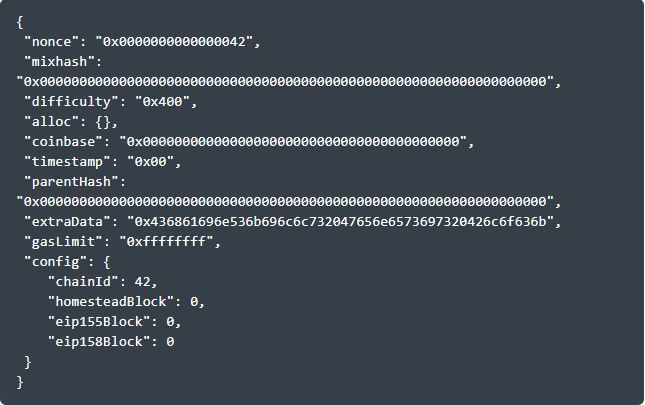
\includegraphics[width=9cm, height=6cm]{genesis.JPG}
  \caption{genesis.json}
  %\label{fig:genesis.json}
  \label{fig:1}
\end{figure}       
  \end{itemize}
  
\begin{enumerate}
\item  \textbf{Initialize miner} 
  
Use the following commands to create the blockchain for the Vendor Node miner.\\
Move to the folder 'VendorNode' just created in the terminal. Then type the following command.\\
\textbf{ geth --datadir $\sim$/VendorNode/miner init genesis.json} \\
   
If you list the content of the miner folder, you will notice the following sub-folders:\\
\begin{itemize}
\item \textbf{geth}: contains the database of your private blockchain (chaindata)
\item \textbf{keystore}: location of your wallet used to store the accounts that you will create on this node.\\
\end{itemize}
%\end{enumerate}

\item \textbf{Creating Accounts} \\
The account will receive all ethers created by the miner in the private blockchain. Type the following command to create a new account\\
\textbf{geth --datadir $\sim$/VendorNode/miner account new}\\

 
 To list all accounts of your node, use the following command:\\
 \textbf{geth --datadir $\sim$/VendorNode/miner account list}\\
 
\item \textbf{Prepare the Miner Nodes} \\
\underline{Miner: setup}\\
\hspace*{1cm} Let’s start by creating a file that will contain the password for our default account, which is the first account we created for each miner. Create a password.sec file under $\sim$/VendorNode/miner/ that contains the password you configured for the first account on miner, in plain text.\\
\hspace*{1cm}   To start the miner, we will require to run the following command:\\ \\
\textbf{ geth --identity "miner" --networkid 42 --datadir "$\sim$/VendorNode/miner" --nodiscover --mine --rpc --rpcport "8001" --port "30303" --unlock 0 --password $\sim$/VendorNode/miner/password.sec --ipcpath "$\sim$/.ethereum/geth.ipc"}\\

You can observe the terminal looks like as shown in   
Fig.\ref{fig:2} \\
  
The meaning of the main parameters is the following:

\begin{itemize}
\item \textbf{identity:} name of our node
\item  \textbf{networkid:} this network identifier is an arbitrary value that will be used to pair all nodes of the same network. This value must be different from 0 to 3 (already used by the live chains)
\item \textbf{datadir:} folder where our private blockchain stores its data
\item \textbf{rpc and rpcport:} enabling HTTP-RPC server and giving its listening port number
\item \textbf{port:} network listening port number, on which nodes connect to one another to spread new transactions and blocks
\item \textbf{nodiscover:} disable the discovery mechanism (we will pair our nodes later)
\item \textbf{mine:} mine ethers and transactions
\item \textbf{unlock:} id of the default account
\item \textbf{password:} path to the file containing the password of the default account
\item \textbf{ipcpath:} path where to store the filename for IPC socket/pipe
\end{itemize}
\hspace*{1cm}To start \href{https://github.com/ethereum/mist/releases}{\textbf{Mist}} browser in private mode, after downloading mist version, run the following command.\\
     \textbf{ ./mist --networkid 42 --rpc $\sim$/.ethereum/geth.ipc}\\
    
    
\begin{figure}
  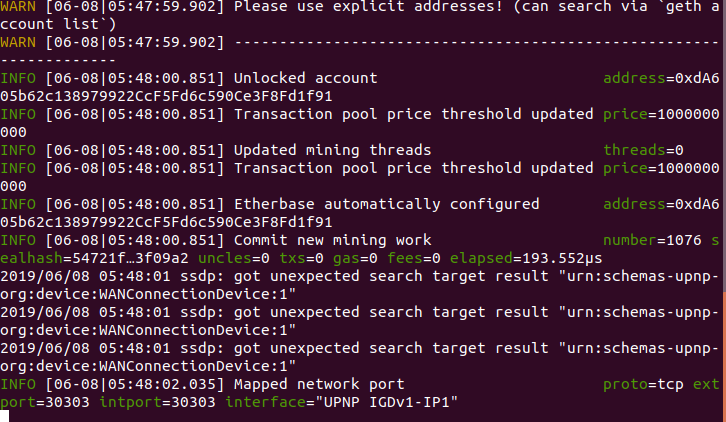
\includegraphics[width=9cm, height=4cm]{run.png}
  \caption{Starting miner1}
  \label{fig:2}
\end{figure}       
  
Note that the ipcpath is the path where you saved your mist application.

\item \textbf{Miner's JavaScript console}\\
Manage your miner using the javascript console.\\
This console needs to be attached to a running instance of Geth.
Open a new terminal session and type:\\
\textbf{geth attach $\sim$/.ethereum/geth.ipc}

This ipc path is shown in the terminal after you run the miner. \\

Repeat the same procedure for the Passive Node on the same or other PC.\\
If you are using the same PC, neglect the ipcpath for the second miner node. It will automatically take \textbf{./miner/geth.ipc} as the default ipc path.

\item Check Balances of the created accounts\\
All these functions are performed in the javascript console.
\begin{itemize}
\item Get the default account with \textbf{eth.coinbase}
\item List the accounts with \textbf{eth.accounts}:
\item To start mining process : \textbf{miner.start()}
\item To stop mining process : \textbf{miner.stop()}
\item To view balance: \\ \textbf{eth.getBalance(eth.accounts[0])}
\item To send ethers from one account to another: \\ \textbf{eth.sendTransaction({from: eth.accounts[0], to: eth.accounts[1], value: web3.toWei(10, "ether")})}
\end{itemize}
\end{enumerate}
\subsection{SYNCHRONISING THE CHAIN}
Here we have to synchronise the network we have created.This is important if we want the transaction to be reflected in the nodes involved.Else they are similar to separate entities.\\

\begin{enumerate}
\item Obtain the ip adrresses of the Vendor and Passive nodes.(Depending on whether its wired or wireless).

\item Start the nodes(both Vendor and the Passive nodes in laptop.Obtain the node information by opening their \textbf{javascript console} and typing the following command:\\ 

\textbf{admin.nodeInfo.enode}\\

\item Create a file \textbf{static-nodes.json}.It contains the node information you just extracted.Replace the placeholder [:] with the IP address of our computer. The last part (?discport=0) has been removed.Each node information is separated by a comma character which can be observed in Fig: \ref{fig:3}\\

 \begin{figure}
  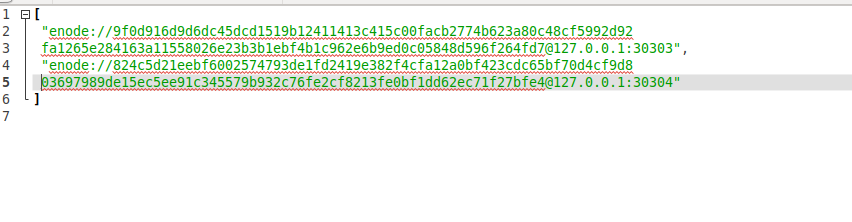
\includegraphics[width=9cm, height=5cm]{static.png}
  \caption{static-nodes.json}
  \label{fig:3}
\end{figure} 


It must be stored under\\
1. $\sim$/VendorNode/miner\\
2. $\sim$/PassiveNode/miner\\


All folders should contain the same file.\\

 

\item Restart the nodes to start the synchronising process.You can see a line in your terminal \textbf{Block synchronising started}.

\item Checking the synchronisation
 Check from PassiveNode:\\
 Open the Javascript console. Type \textbf{admin.peers} in the console and observe the results.\\
 We can see that our node is paired to VendorNode miner  identified by its IP address and its port number(30303). Similary try this on other node, to check if its connected.\\
 
\item Try sending ethers from one node to another to understand the working.\\
 \textbf{eth.sendTransaction(\{{from: eth.accounts[0], to: "0xae3ab39b3ebc425289dad620aece197\\a4a3f8940", value: web3.toWei(2, "ether")\}})} \\
 
If you have more than one account, you have to unlock those accounts to be able to send transactions to it.\\
 
\textbf{personal.unlockAccount(eth.accounts[1], 'type your password')}
\end{enumerate}


\subsection{CREATING AND DEPLOYIND SMART CONTRACTS}
We create a simple contract called 'MedRec'. This contract will hold an associative array of unique integers and Patient objects. Here, the unique integer we considered is Aadhar Number.\\

\begin{enumerate}
\item Installing Truffle
A developmental framework for Ethereum, we use truffle to create and deploy smart contract.\\
\textbf{ npm install -g truffle} \\
\textbf{Note:} Install \textbf{node-js} and \textbf{npm} before the installation of \textbf{truffle} framework if you didn't installed earlier.
\item Installing Node.js from NodeSource repository
\begin{itemize}
\item sudo apt-get install curl
\item \$ curl -sL https://deb.nodesource.com\\/setup\_10.x $\mid$ sudo bash -
\item \$ sudo apt-get update
\item  \$ sudo apt install nodejs

Check the version of node-js and npm:\\
\textbf{pi\$ node -v}\\
\textbf{pi\$ npm -v}\\
\end{itemize}

 
\item Create the directory that will host your project.\\
\textbf{ mkdir $\sim$/VendorNode/Projects/healthcare}\\
Move to this directory using cd command and type:\\
\textbf{truffle init} 

\item Create a file 'MedRec.sol' in the \textbf{contracts} directory and paste the code shown in the Fig:\ref{fig:4}

 \begin{figure}[H]
  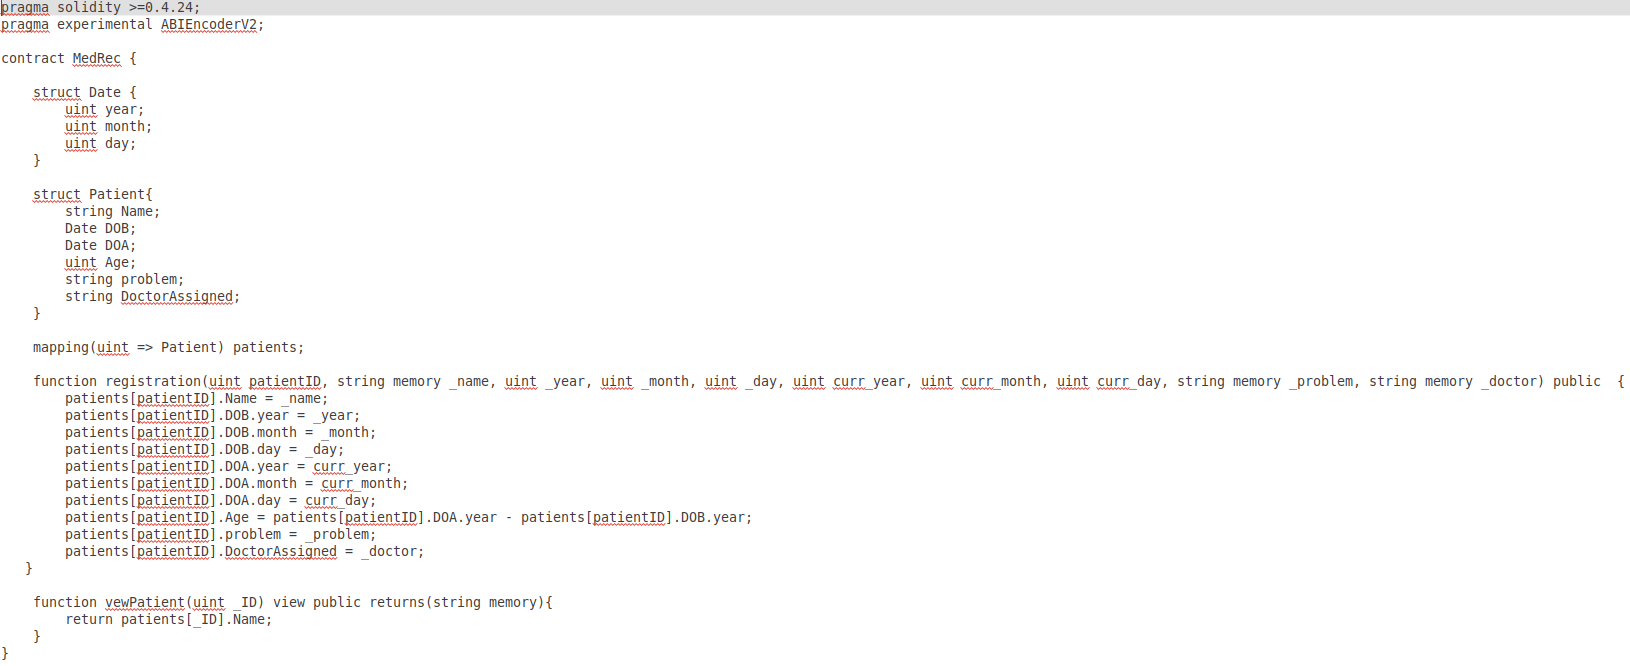
\includegraphics[width=9cm, height=5cm]{smartt.png}
  \caption{MedRec.sol}
  \label{fig:4}
\end{figure} 

 \item Go to the \textbf{migrations} directory and create a file \textbf{2\_deploy\_contracts.js} with the content shown in Fig:\ref{fig:5}
 
  \begin{figure}[H]
  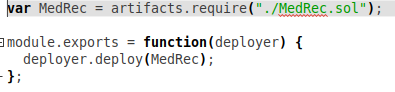
\includegraphics[width=8cm, height=2cm]{deploy.png}
  \caption{2\_deploy\_contract.js}
  \label{fig:5}
\end{figure} 
 
 \item create a file \textbf{truffle-config.js} or edit if already present and set the network conditions as shown in Fig:\ref{fig:6}\\
 
  \begin{figure}[H]
  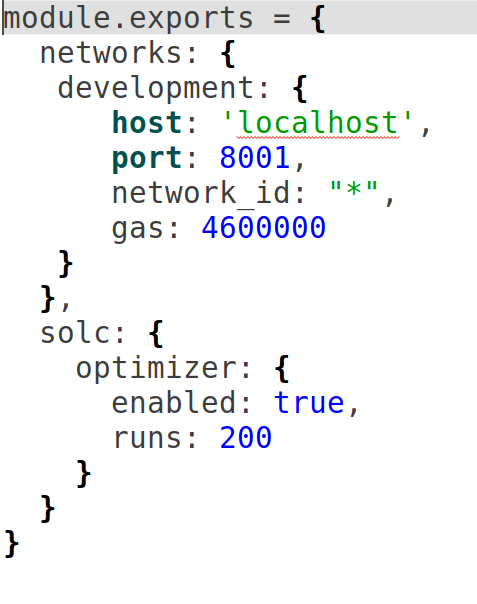
\includegraphics[width=8cm, height=6cm]{truffle.png}
  \caption{truffle-config.js}
  \label{fig:6}
\end{figure} 

 \item Start your miners before proceeding to the deploying process.
 
 \item \textbf{\$ cd $\sim$/VendorNode/Projects/healthcare}

       \textbf{\$ truffle compile}

       \textbf{\$ truffle migrate --reset} \\
Now our SmartToken contract is deployed onto our private Ethereum chain and it is ready to receive calls.

 \item Identifying your Contract\\
We have to retrieve two elements about our deployed contract:its address
and its ABI (Application Binary Interface).

\item Open truffle console: \textbf{truffle console}

\item Obtain contract address: \textbf{MedRec.address}

\item obtain ABI: \textbf{ JSON.stringify(MedRec.abi)}

%\item Download mist for linux and extract it.

\item Move the \textbf{$\sim$/Mistt} and start mist using the command:\\
\textbf{./mist --networkid 42 --rpc $\sim$/.ethereum/geth.ipc}
Make sure it opens in your private network and not to the main-net.
\item Open \textbf{Watch Contract}. Fill in the smart contract address and ABI.
Now the smart contract is available on Mist and you can easily interact with it. 
\item You can copy the smart contract address and ABI on the mist browser running on the PassiveNode.

\begin{figure} 
  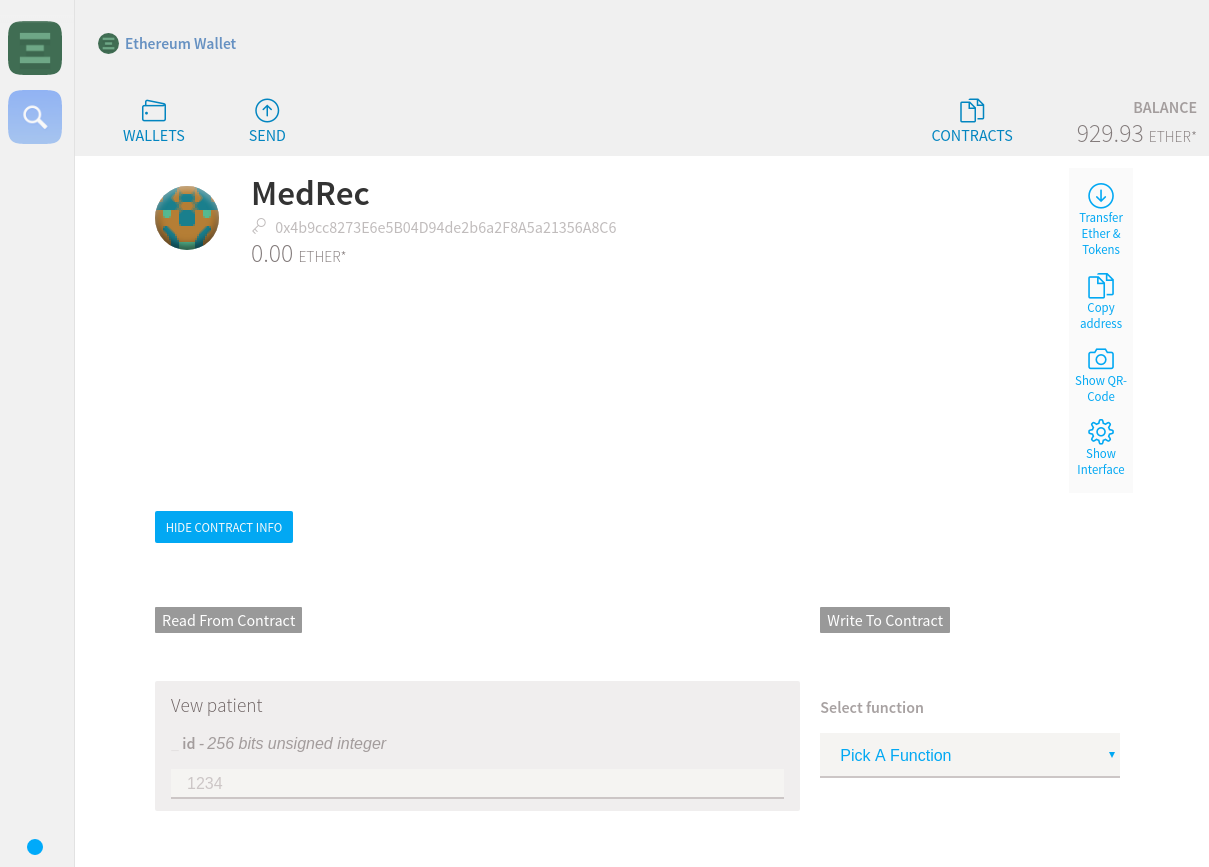
\includegraphics[width=9cm, height=6cm]{mist.png}
  \label{fig:7}
  \caption{Mist Browser Screen}
\end{figure} 
\end{enumerate}

\subsection{CREATING THE CLIENT-SIDE CODE}

\begin{enumerate}

 \item Create a file \textbf{package.json} under healthcare directory with the code shown in Fig:7

  \begin{figure}[H]
  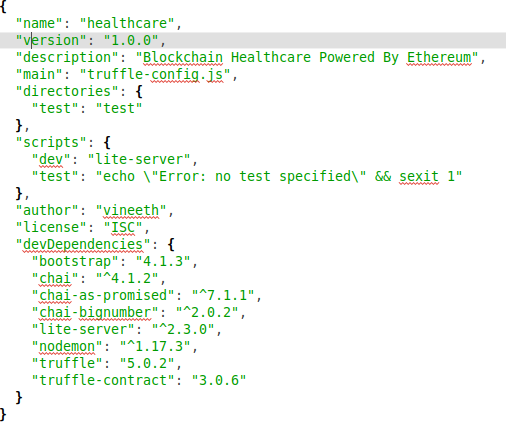
\includegraphics[width=8cm, height=8cm]{package.png}
  \caption{package.json}
  \label{fig:8}
  \end{figure}

 \item \textbf{\$ npm install}

 \item Create files \textbf{src\//index.html, src\//app.js}
 
 \item Create a file named \textbf{bs-config.json}\\
 We are using \textbf{lite-server} to serve all of the project files for the client side. We'll need to tell \textbf{lite-server} where all these files are located. We can do this by updating the browsersync configuration for \textbf{lite-server} inside the \textbf{bs-config.json} file. Paste this configuration into your project file:
 
  \begin{figure}[H]
  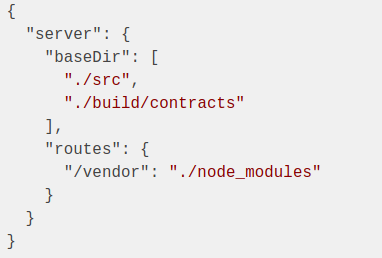
\includegraphics[width=6cm, height=5cm]{config.png}
  \caption{bs-config.json}
  \label{fig:9}
  \end{figure}
  
  This configuration tells lite-server to expose all the files in the src and build/contracts directories to the root of our web server. It also adds an alias for any files in the node\_modules directory to appear in the vendor route. This will allow us to pull in any project dependencies like bootstrap into the client side with the vendor route, which we'll see momentarily.
  
  \item Paste the following code from github in \href{https://github.com/vinnoo/healthcare/blob/master/VendorNode/Projects/healthcare/src/index.html}{index.html}
  \item Paste the following code from github in \href{https://github.com/vinnoo/healthcare/blob/master/VendorNode/Projects/healthcare/src/app.js}{app.js}
  
  \begin{itemize}
      \item \textbf{loadWeb3():} web3.js is a JavaScript library that allows our client-side application to talk to the blockchain. We configure web3 here. This is default web3 configuration specified by Metamask.
      
      \item \textbf{loadContract()} This is where we load the smart contract data from the blockchain. We create a JavaScript representation of the smart conract wit the Truffle Contract library. Then we load the smart contract data with web3.
      
      \item \textbf{register()} This is where we retrieve the data from the webpage and send it to the solidity function \textbf{registration(),} which will allow us to write the data to the blockchain.
  \end{itemize}
  
  \item \textbf{\$ npm run dev}\\
  Now the webpage is loaded. But, you will see errors in the browser console.\\
  \begin{figure}[H]
  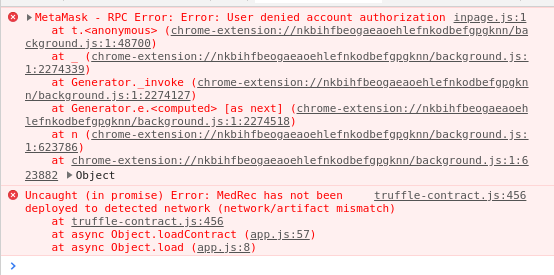
\includegraphics[width=8cm, height=5cm]{error.png}
  \caption{Errors in the browser console}
  \label{fig:10}
  \end{figure}
  
  That's because, you need to connect to one of the accounts that you have created before with the metamask extension.
  You can get the metamask extension from the link: \href{https://chrome.google.com/webstore/detail/metamask/nkbihfbeogaeaoehlefnkodbefgpgknn}{\textbf{Metamask}}
  
  \item Now, we need to connect to the account and the hosted network \textbf{(http://127.0.0.1:8001)} with the metamask, where, 127.0.0.1 is the \textbf{localhost} domain and \textbf{8001} is the port that we configured in \textbf{truffle-config.json} file.
  
  \item The private key to the account can be obtained by using the python code as shown in the figure Fig. 10.
  
  \begin{figure}[H]
  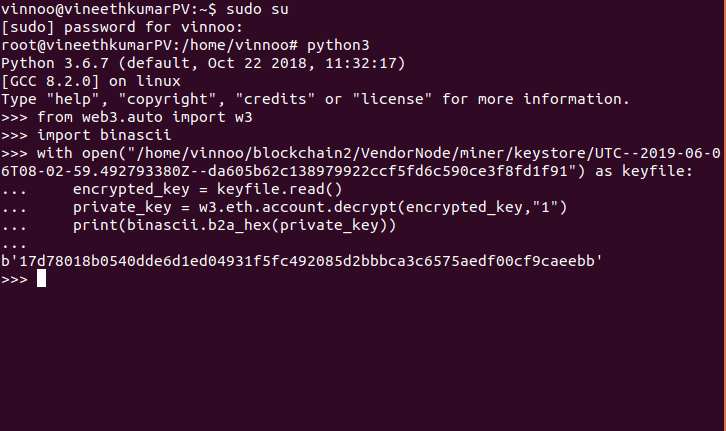
\includegraphics[width=8cm, height=5cm]{private.png}
  \caption{Private Key Extraction}
  \label{fig:11}
  \end{figure}
  
  Now, create a custom rpc with new rpcurl as \textbf{(http://127.0.0.1:8001)}
  
  \item Reload the browser to see the account loaded at top right corner of the page and the errors in the browser console subside.

\end{enumerate}

\subsection{WORKING}
 \begin{enumerate}
     \item Enter the details on the webpage and click on submit button. Then, you will receive a pop-up, asking for confirmation.
     \item Click confirm.
     \item Start the mining process for the transaction to get confirmed.
     \item After confirmation, you can then confirm the process using \textbf{Mist} browser.\\
     \textbf{./mist --networkid 42 --rpc $\sim$/.ethereum/geth.ipc}
     \item Enter the Aadhar number you entered before, in the VewPatiet function. It will return the Name of the patient.
 \end{enumerate}

\subsection{CONCLUSIONS}
You can test your applications using Mist browser by deploying your own Dapps(Smart contracts) on your private ethereum nodes. 

\begin{thebibliography}{99}
\bibitem{c1} Mastering Blockchain: Distributed ledger Technology, decentralization and smart contracts ($1^{st}$ Edition) by Imran Bashir 
\bibitem{c2} http://chainskills.com/2017/02/24/create-a-private-ethereum-blockchain-with-iot-devices-16/.
\bibitem{c3} https://bitfalls.com/2018/03/25/run-private-ethereum-blockchain/.
\bibitem{c4} https://github.com/trufflesuite/truffle/issues/305

\end{thebibliography}
\end{document}
